\documentclass[letterpaper,12pt]{article}
\usepackage[utf8]{inputenc}
\usepackage{fullpage}
\usepackage{courier}
\usepackage[margin=0.75in]{geometry}
\usepackage{listings}
\usepackage{color}
\usepackage{graphicx}
\usepackage[width=5in]{caption}
\usepackage{hyphenat}

% Format a sectionless paragraph
\newcommand*\unparagraph{
	\par
	\nopagebreak
	\vskip3.25ex plus1ex minus.2ex
	\noindent
}

% define extra colors
\definecolor{dkgreen}{rgb}{0,0.6,0}
\definecolor{purple}{RGB}{159,0,197}

% define the code listing format
\lstset{
	language=C++,
	basicstyle=\footnotesize\ttfamily,
	backgroundcolor=\color{white},
	showspaces=false,
	showstringspaces=false,
	frame=none,
	tabsize=3,
	keywordstyle=\color{purple},
	commentstyle=\color{dkgreen},
	stringstyle=\color{blue},
	escapeinside={\%*}{*)}
}

% efine the title/header
\title{\Large CS 1428\\Lab 11 Sections L19 and L06} 
\author{Jared Wallace}
\date{}

\begin{document}

\maketitle

\vspace{30mm}

\section*{Passing arrays to functions}
Today we are discussing the nuances of passing arrays to functions. We like to say
that arrays are passed by reference.  This is not strictly true but it is true enough
for our purposes and if you continue on to CS 2308 you will learn more detail. When 
we prototype a function that is going to receive an array we have to specify that the
parameter is an array of some type rather than that type itself.  We do this using the
square braces $[]$.

\begin{lstlisting}
void fillArray(int array[], int size);
\end{lstlisting}

The braces are only there to signify to the compiler that we are passing an array, 
they are not the same as the braces we use when accessing a specific element within
an array.  When we call this function we pass the array by name only. This is because 
we want to pass the entire array, not any specific element.

\begin{lstlisting}
int main() {
	int array[] = {1,2,3,4,5};
	fillArray(array, 5);
}
\end{lstlisting}

The function itself will take the name passed in and it can index that array name the
same way it would if the array had been declared as a local variable.  Just like when
we pass a variable by reference, any changes that are made to the array will be persistent
in the calling function (in our case this will always the main function, but if you recall
we discussed that functions can call other functions).

\begin{lstlisting}
void fillArray(int array[], int size) {
	for (int i = 1; i <= size; ++i)
		array[i] = i;
}
\end{lstlisting}

\section*{Program}
We are going to create a program that passes a single array around to several different
functions.  Each function will alter the array moving us closer to our goal. It is in
your best interest to write each function in order as they are requested.  Take it one
step at a time.

\begin{enumerate}
	\item Start by including the headers you will need to print to the screen, read from
		and write to files and manipulate the format of output text. You should also go ahead
		and create an empty main function.
	\item We are going to read in and process an unknown number of grades from a file. We are
		placing an upper limit of 100 possible grades so that we know how large to make our 
		actual array and so we can prevent an overlarge file from crashing our program. You
		should declare a global constant now set to the value 100. You should also create a 
		global constant for the filename. Note: Constant c-strings must be declared in a particular
		way: \lstinline$const char* NAME = "some string";$
	\item First create a function that will read read the grades from a file. This function
		should take exactly two parameters.  The first is our array of grades and the second
		is a counter. The array is passed by reference automatically, the counter can either
		be passed by reference or the value can be returned. You should be familiar with both
		of these options and may pick whichever you prefer (there is no ``right'' answer). Loop
		through the file and read grades until you encounter an invalid grade. This is the 
		sentinel telling you when to stop. Don't forget to increment your counter.
	\item The teacher is benevolent and wishes to apply a curve. You need to write a function to
		apply this curve. The parameters this function needs are the array itself and the counter. 
		First you should loop through the entire array searching for the lowest value.  
		\begin{itemize}
			\item Start by assuming that the first value is the lowest. Then loop through the array
				starting with the second item checking each value to see if it is lower than the one
				we currently believe to be the lowest. If it is, update your lowest value and continue.
			\item Calculate the value of the curve to be applied.  This is 70 - lowest grade.
			\item Loop through the array again applying the curve. Each grade should be increased by
				the value of the curve. Each time you increase a grade verify that it does not exceed 
				100.  If it does, the grade should be set back to a maximum of 100.
		\end{itemize}
	\item Next we need to calculate the final average of all grades for the teacher.
		This should be a familiar exercise by now. Loop through the array one last time calculating 
		the total sum. Divide that sum by the counter to get the total average and return it.

\newpage
   \item The last function I have written for you, in the interest of making your life a bit easier.
      You shouldn't have to mess with this at all.
	\item The last thing to do is to add the meat to your main function.  Create the variables
		you need and call each function in the order they were listed. TEST your program!

\end{enumerate}

\vspace{15mm}

% Don't forget the submission instructions!
\unparagraph{} \textbf{The source code should be printed out and stapled to the back of this
	sheet as well as uploaded to the server.}

	\vspace{25mm}

% Comic at the bottom
\begin{figure}[ht!]
	\centering
	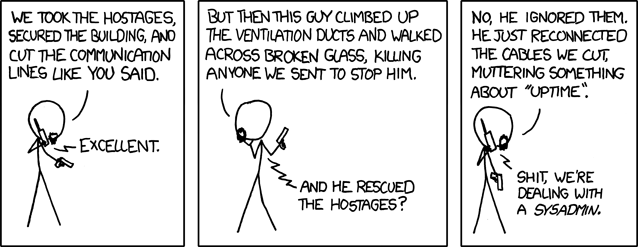
\includegraphics[width=5in]{devotion_to_duty.png}
	\caption*{The weird sense of duty really good sysadmins have can border on the sociopathic, 
		but it's nice to know that it stands between the forces of darkness and your cat blog's servers.}
\end{figure}

\end{document}
